\documentclass[11pt]{article}
\usepackage{graphicx}
\usepackage[margin=1in]{geometry}
\usepackage{mathtools}
\usepackage{hyperref}
\linespread{1.5}
\title{\textbf{Self Organizing Maps \& CUDA}}
\author{Doug Woodward}
\date{}
\begin{document}

\maketitle
\begin{center}
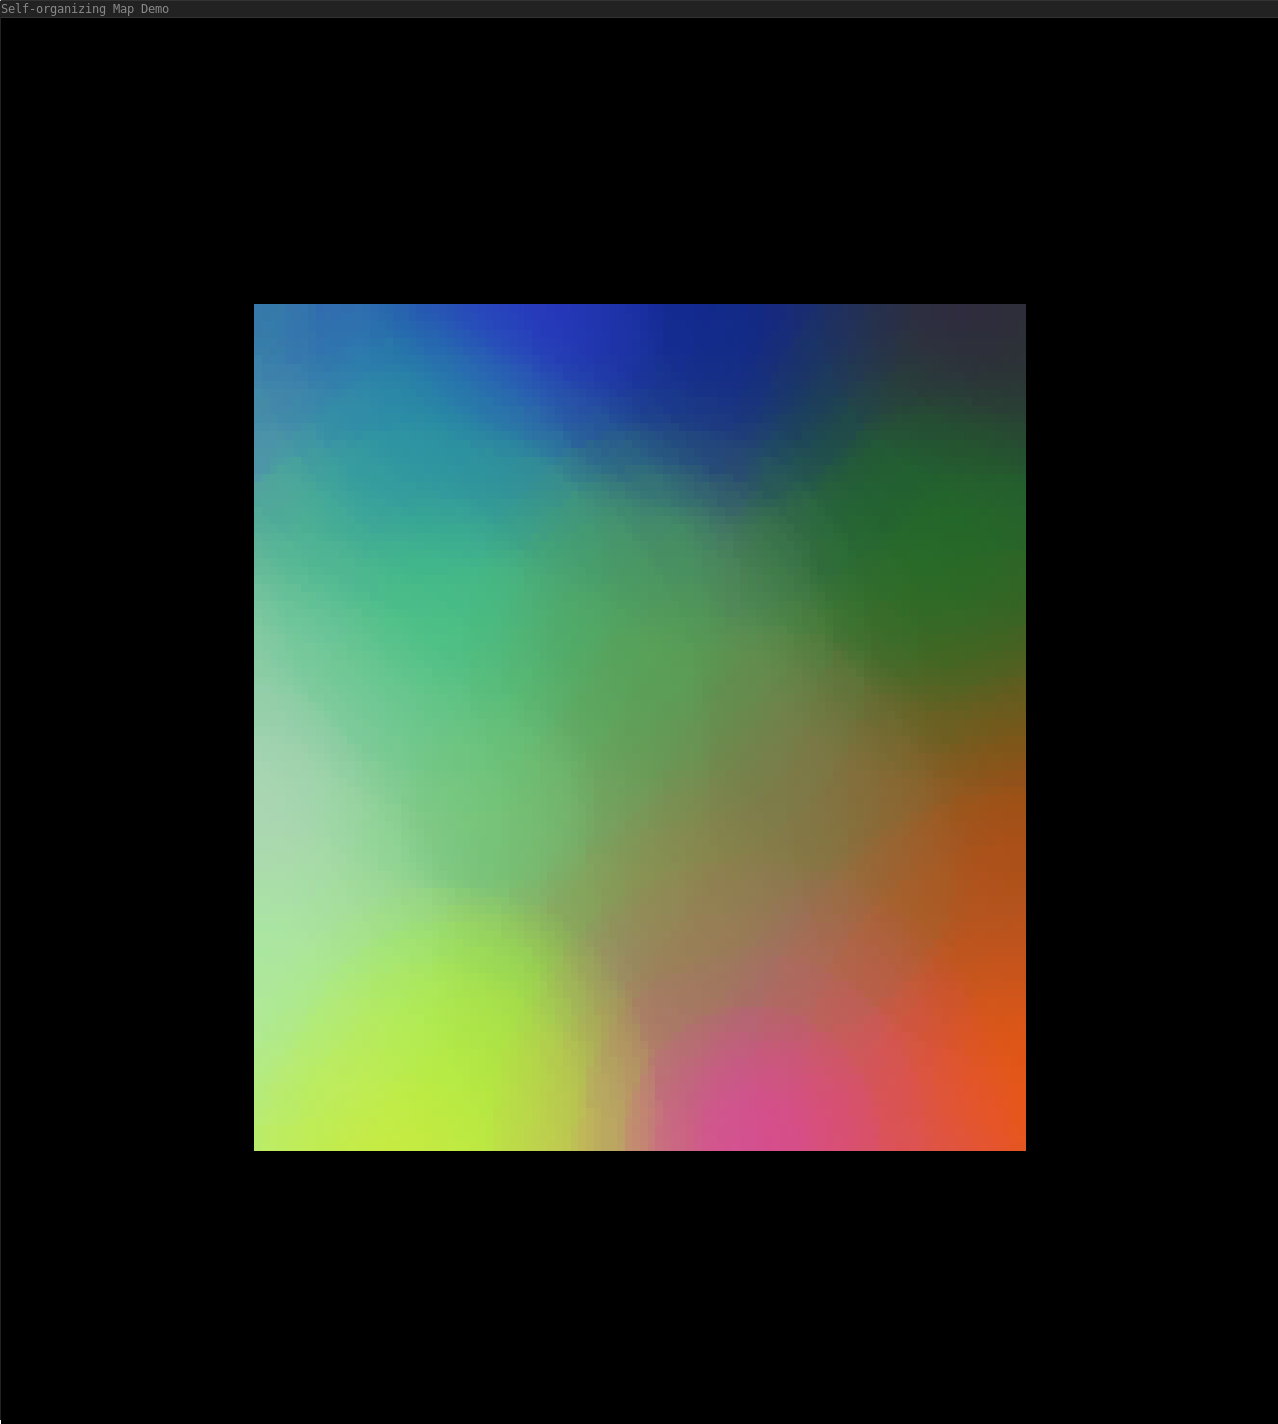
\includegraphics[scale=.15]{title}
\end{center}
\section{Introduction}

Self Organizing Maps are a type of clustering, unsupervised neural network well suited to visually displaying information that exists in higher dimensional spaces down into two and three dimensional space such that a human observer can interpret it intuitively. Self Organizing Maps preserve the topological relationships of high dimensional data when compressing down into lower dimensional space. SOMs are frequently used in meteorology, oceanography, prioritization, and even in the creation of artwork - an unexpected use to be sure, but one that even this project gives credit to in the distributions of colors when adjusting parameters. This paper seeks to explore the parallelization of a SOM algorithm using CUDA to leverage the high throughput capability of GPUs.

In this paper, the data the SOM is trained on is fairly trivial, RGB color points - three dimensional data that will be clustered in two dimensional space. However, the algorithm and implementation herein can be converted with minimal effort to handle more complex data - for example, RGBA values or even data points with hundreds of attributes. The key requirement is that there exists a method of distance calculation between two points.
\section{SOM Implementation}
Implementing a SOM can be broken down into the following steps:
\begin{enumerate}
\item{Initialization}
\item{Sampling}
\item{Matching}
\item{Updating}
\item{Repeat}
\end{enumerate}
\subsection{Initialization}
The initialization of a SOM can have a significant influence on the end result and the time taken to train the algorithm. In this project, the data is initialized as a \(N \times M\) matrix of RGB points where the RGB values of each points are generated randomly. The initialized, untrained map is below.
\begin{center}
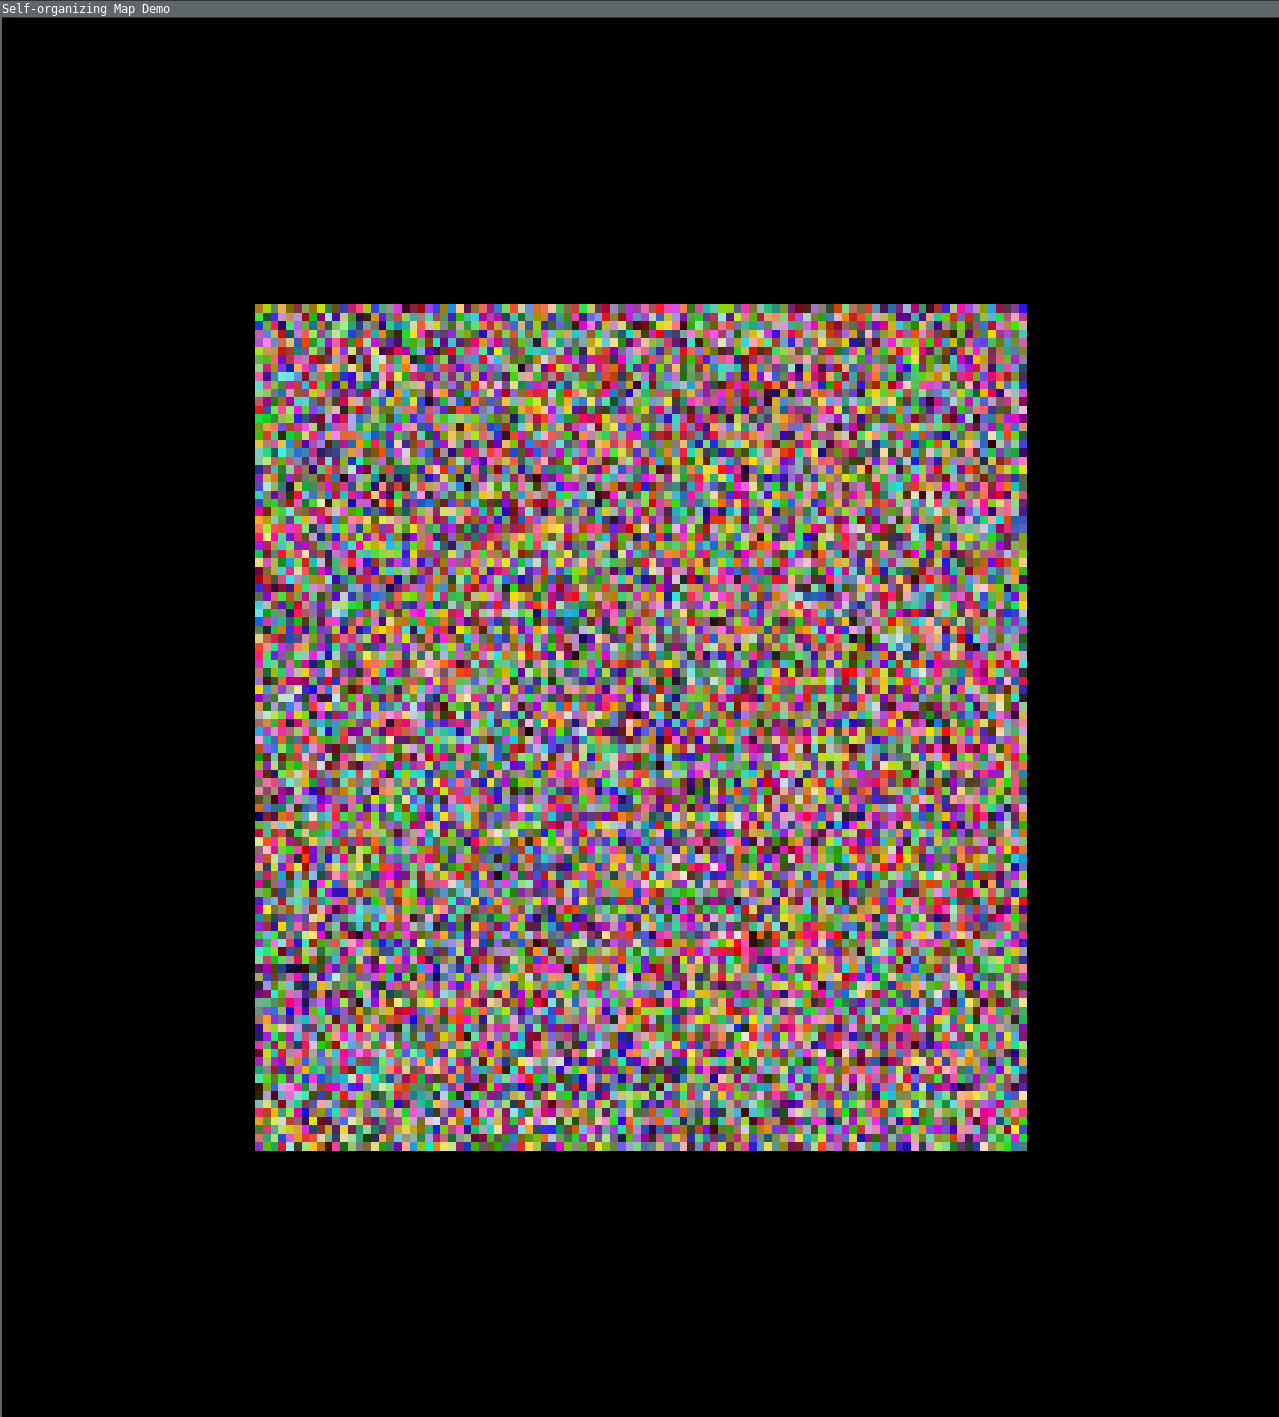
\includegraphics[scale=.15]{cuda_som_init}
\end{center}
Each time the map is initialized the points are assigned RGB values at random, resulting in even the same training data set producing differing outputs in the overall arrangement. That is not to say the clustering is any different, nor does the relative arrangement of clusters change, but the entire SOM may be rotated or transformed as below. 
\begin{center}
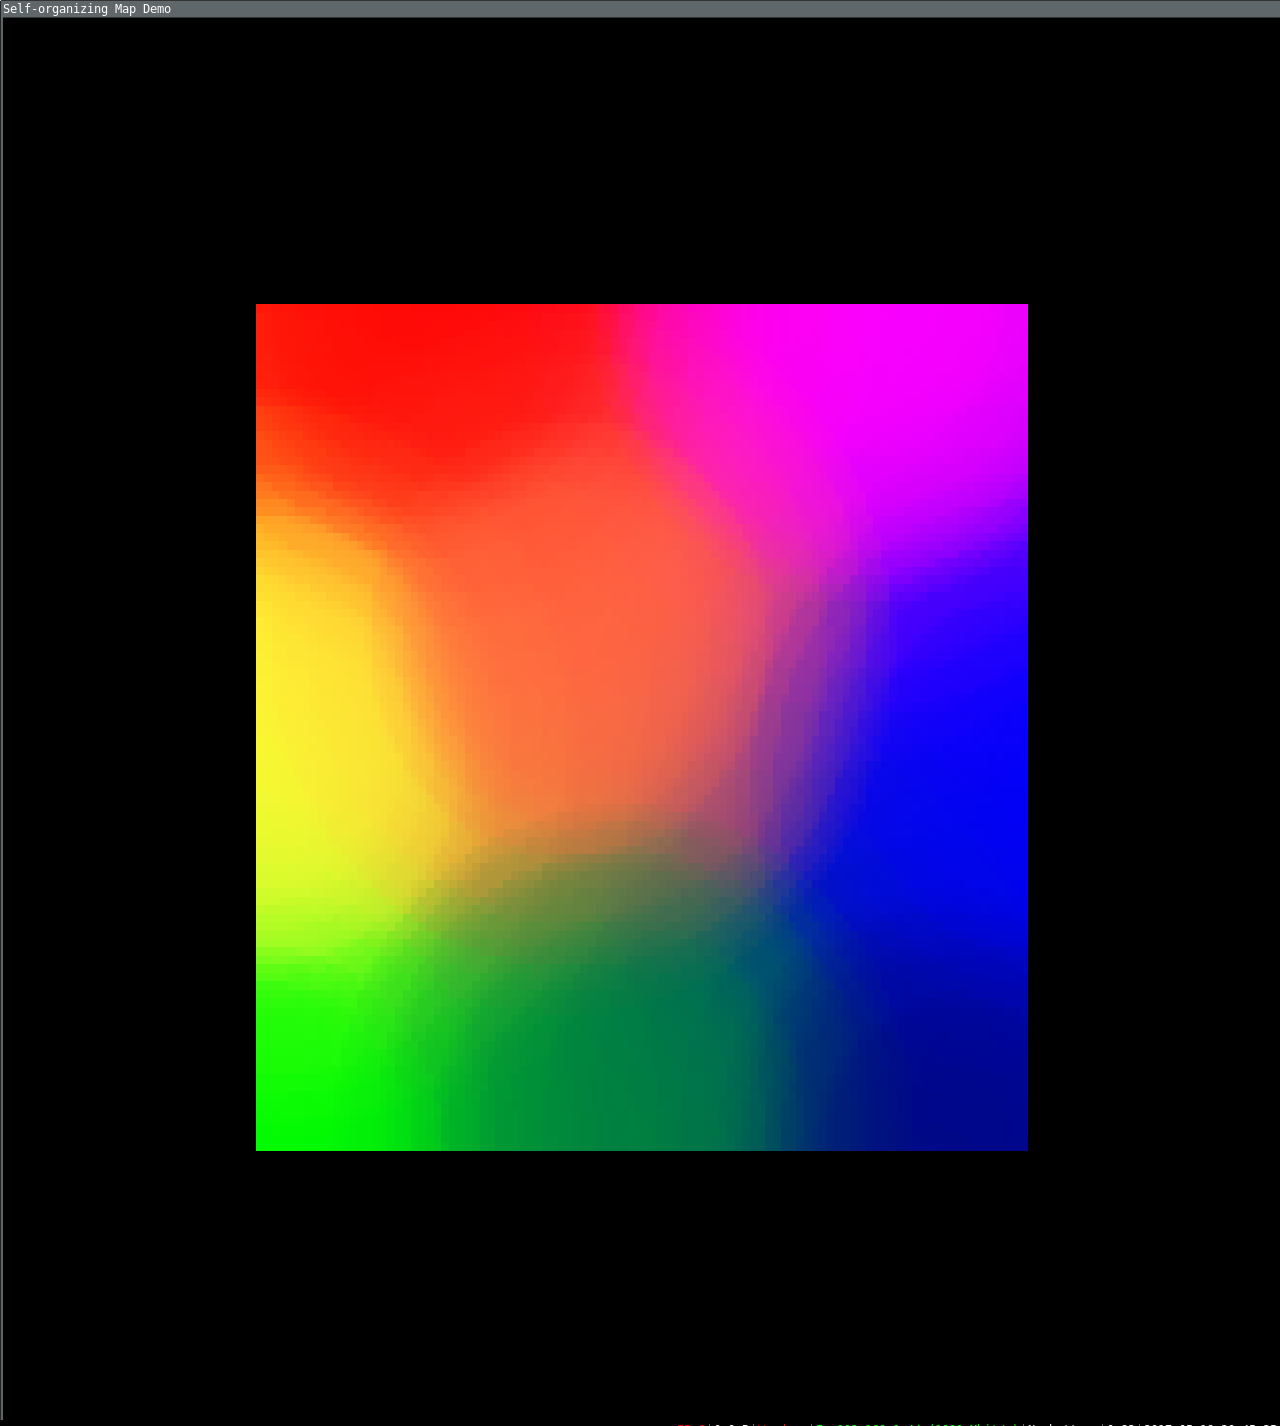
\includegraphics[scale=.15]{output1}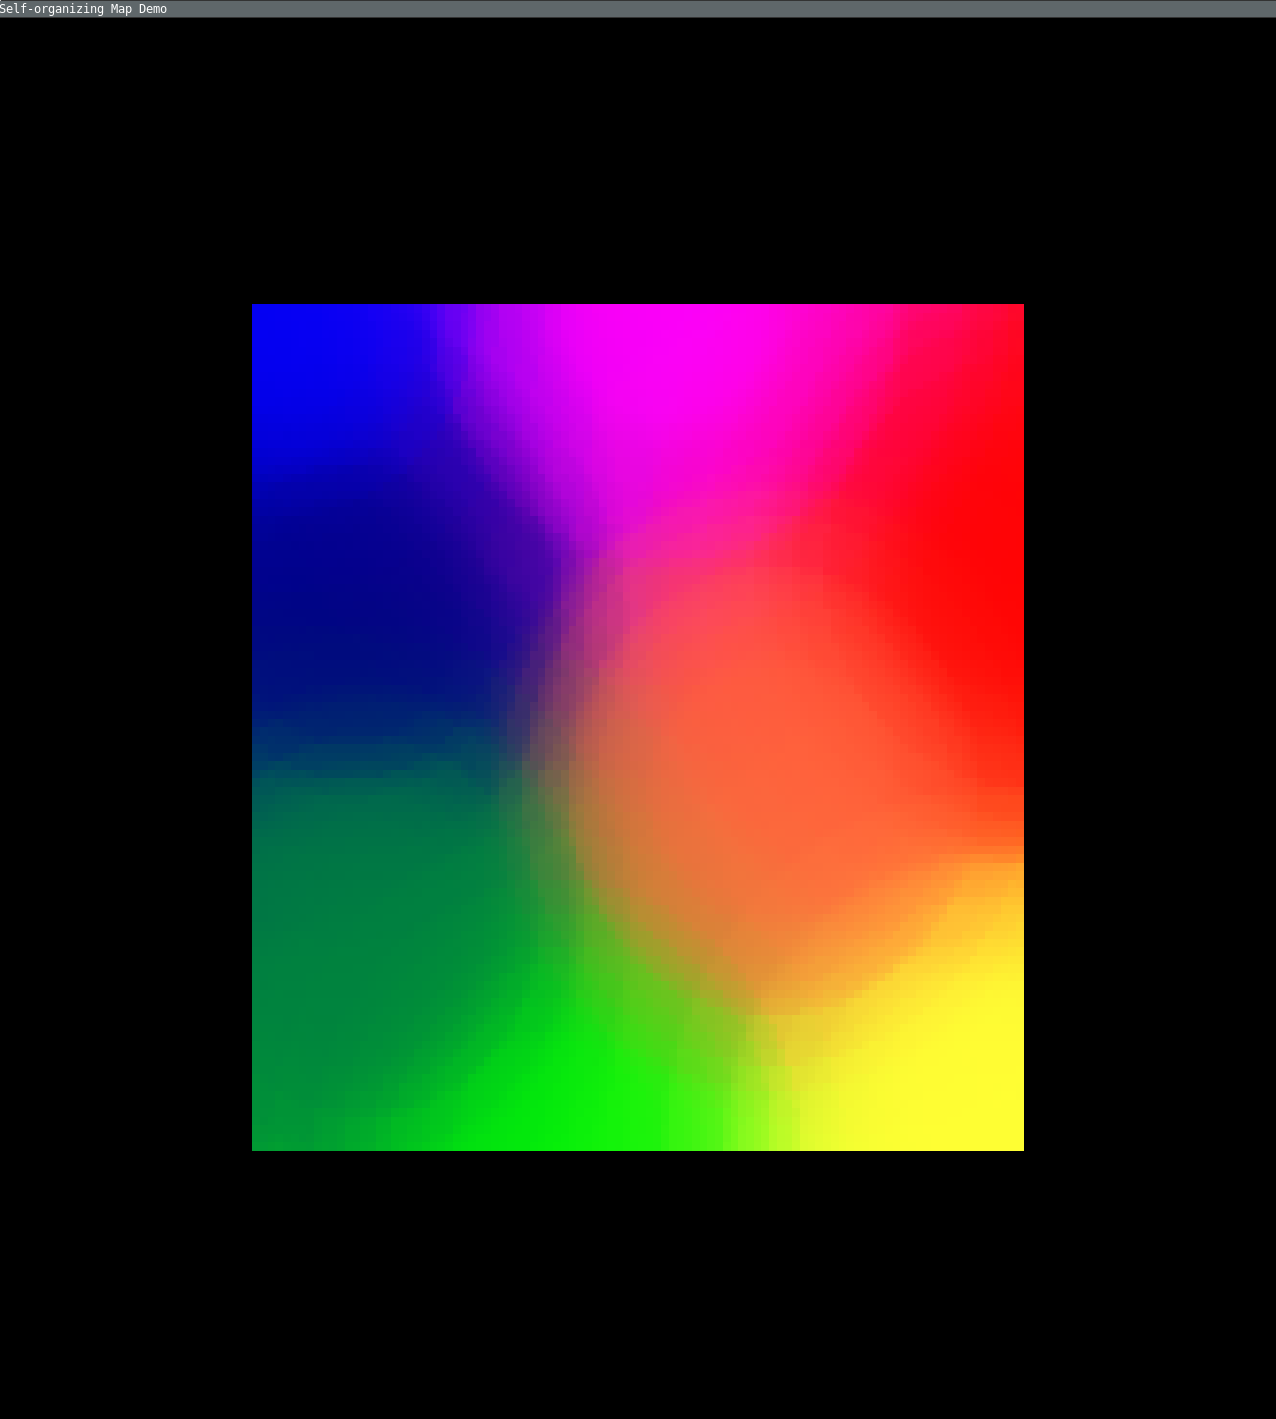
\includegraphics[scale=.1505]{output2}
\end{center}
This variance is explained by the algorithm selecting the closest match for each input data point and adjusting the surrounding weights accordingly, with random initialization of the map, the closest point to say Dark Blue, could be anywhere on the map to start, top left, bottom right etc. However, orange always clusters to the center as the map retains the topological relationships between clusters in lower dimensional space.

\subsection{Sampling}

The sampling step is a fairly straightforward process, from the training data, a point is selected at random to be input into the map. Of note here, the random selection has no more bearing on the final result than the random initialization, it may affect the rotation or transformation but can not effect the topological relationships.

\subsection{Matching}

Here, the need for a distance formula specific to the data set arises. Within the scope of this paper, a simple Euclidean Distance formula is used: \begin{math}\sqrt{\sum\limits_{i=0}^{i=n} ({p^1_i}-{p^2_i})^2} \end{math}  where \(p^1\) and \(p^2\) are two RGB color points. For other data sets, more complex distance formulae may be necessary. Once the best match is chosen, the algorithm proceeds to the next step. Because of the need to process the same simple equation on many points when each individual calculation has no bearing on the others, this section of the algorithm was targeted for parallelization.

\subsection{Updating}

Following the selection of the best matching point, the points surrounding the best match must be updated as well, with the magnitude of the decrease scaling inversely with the distance from a node and also influenced by the learning rate, which typically decreases over the life of the training. To have the radius of influence shrink with time an exponential decay function is used. \begin{math}\sigma_0exp(-t/\lambda) \end{math} where \(\sigma_0\) is the half the width of the map, \(t\) is the time step, and \(\lambda\) is the learning rate which is equivalent to the current number of iterations over the log of half the width of the map. 

\subsection{Repeating}

The algorithm repeats the above steps until some break condition is met. For this project, the break conditions are that set are a certain number of iterations, 1000, or if the total change induced in the map by a data point is less than 0.1.

\section{Parallelization with CUDA}

In applying parallelization to the algorithm, the matching step was the most viable candidate for optimization. Adjusting the code to accommodate a Cuda kernel call required more effort than dropping an OpenMP section into the code. One notable restriction of CUDA is the lack of more sophisticated data structures, which limits the ability to apply an object oriented approach to a CUDA program. This also meant that the nested std::vector data structures employed needed to be flattened into a one dimensional array of doubles to be used by the CUDA kernel call. This meant that the entire matrix became an \(N \times M \times 5\) length pointer and the vector of distances for each node in a comparison became an \(N \times M\) array. Because of this length mismatch, the indexing required some adjustment based on the thread id such that the index for the flattened map was multiplied by 5 during the interior loop of the kernel over RGB values. 


Once the step was identified and some of the data structure mismatches resolved, the kernel was employed to calculate the distance for each node to the training point. After the kernel ran and the data was transferred back to the host, the thrust::min\_element method was used to find the index of the smallest distance. Once the point was chosen, the weights were adjusted serially. An effort was made to parallelize the weight updates as well, however this was unsuccessful in large part due to project being built serially first.


Unfortunately, there was no speedup realized by the implementation of CUDA in this algorithm. That is not to say that a Self Organizing Map can not be parallelized to take advantage of GPU processing power, rather that the implementation of the SOM in this project was an ill suited match for it. The results of runs in parallel and serial execution are shown below, note that the training data was controlled for this comparison test.

\begin{table}[!htbp]
\centering
\begin{tabular}{|c|c|c|c|c|}
\hline
	Size & Serial & Parallel \\
\hline
	 \(5 \times 5\) & 8.428 & 8.4907\\
\hline
	 \(10 \times 10\) & 8.507 & 8.366\\
\hline
	 \(100 \times 100\) & 8.396 & 8.943\\
\hline
	\(100 \times 100 \) & 10.10 & 10.266\\
\hline
	\(200 \times 200 \) & 8.701 & 48.2106\\
\hline
	\(300 \times 300 \) & 9.802 & 109.571\\
\hline
\end{tabular}
\end{table}

The data above shows that the algorithm in serial is unaffected by the size of the data, but the CUDA enabled version takes a monstrous hit once the data set is greater than 1000 points, scaling roughly linearly with the data size. This occurs because the bottleneck in a CUDA application is the speed and frequency of transferring data to and from the GPU. Because this program was built first serially, not all parts can be run on a GPU - especially the object oriented portion. Additionally, the program leverages OpenGL through glut, but does not do so on the GPU side. Inside of each epoch of the program, the entire map is transferred to and from the GPU. This is a poor way to leverage CUDA, and the future improvements to the project will seek to shift the entirety of computation to the  GPU and only have one transfer to and one transfer back for the entire program. If this were to be implemented, one would expect that the GPU program would indeed see significant speedup over the CPU as no part of the algorithm is averse to parallelization. 

\section{Conclusion \& Lessons Learned}
The major takeaway from the development of this project is that when implementing an algorithm in CUDA one is much better served to design it specifically for CUDA from the start as opposed to developing the algorithm serially and then converting. Additionally, the cost of transferring data to and from the GPU is clearly highlighted and needs this needs to be minimized as much as possible.

\section{Code}

Code can be found at \texttt{\href{https://github.com/rugggg/CADS/tree/master/CS540/nBody}{https://github.com/rugggg/CADS/tree/master/CS540/som}}

\begin{thebibliography}{9}
\bibitem{cuda} 
Cuda Developer Toolkit
\\\texttt{https://developer.nvidia.com/how-to-cuda-c-cpp}
\textit{nVidia}. 
 
\bibitem{Thrust} 
\texttt{https://thrust.github.io/}
[\textit{Thrust}]. 

 
\bibitem{ai-junkie} 
Kohonen's Self Organizing Feature Maps
\textit{Tom Ventimiglia \& Kevin Wayne}
\\\texttt{http://www.ai-junkie.com/ann/som/som1.html}

\bibitem{barnes-hut} 
Self Organizing Maps: Algorithms and Applications
\textit{John A. Bullinaria}
\\\texttt{http://www.cs.bham.ac.uk/~jxb/NN/l17.pdf}
\end{thebibliography}

\end{document}